\section{Introduction}
\begin{frame}{Introduction}
\begin{justify}
            TheHive is a scalable open source and free Security Incident Response Platform designed to make life easier for SOCs, CSIRTs, CERTs and any information security practitioner dealing with security incidents that need to be investigated and acted upon swiftly.
            \vspace{1em}

            We can synchronize it with one or multiple MISP instances to start investigations out of MISP events. We can also export an investigation's results as a MISP event to help our peers detect and react to attacks we've dealt with. Additionally, when TheHive is used in conjunction with Cortex, security analysts and researchers can easily analyze tens if not hundred of observables.
            
\end{justify}
\end{frame}


\begin{frame}{Introduction continued}
\begin{justify}
            Collaboration is at the heart of TheHive. Multiple analysts from one organisations can work together on the same case simultaneously. For example, an analyst may deal with malware analysis while another may work on tracking C2 beaconing activity on proxy logs as soon as IOCs have been added by their coworker. Using TheHive's live stream, everyone can keep an eye on what's happening on the platform, in real time.
            \vspace{1em}

            So the main purpose of using this tool is to detect any security incident quickly and analyze that incident in a collaborative platform to solve any security issue efficiently.
            
\end{justify}
\end{frame}

\begin{frame}{Source Code Architecture}
\begin{justify}
           \item \begin{justify}
        \textbf{Backend:}TheHive's backend is Written in Scala.The backend is primarily based on the Play Framework.
    \end{justify}

    \item \begin{justify}
        \textbf{Frontend:} TheHive's frontend is built using AngularJS.
    \end{justify}

    \item \begin{justify}
        \textbf{Database:}TheHive primarily used the Elasticsearch search and analytics engine as its data store and indexing solution. Later it used Casandra, a distributed NoSQL database that is typically used for handling large volumes of structured and semi-structured data in a horizontally scalable and fault-tolerant manner
    \end{justify}

    \item \begin{justify}
        \textbf{Documentation and Configuration:}The project is typically well-documented, providing guidance for installation, configuration, and usage.Configuration files are used to customize the behavior of TheHive to suit an organization's specific needs.

    \end{justify}

    
\end{justify}
\end{frame}

\begin{frame}{APIs}
\begin{justify}
    APIs are available for following purposes.
    \begin{enumerate}
    \item Organization
    \item User
    \item Custom field
    \item Case template
    \item Alert
    \item Case
    \item task
    \item Observable

    \end{enumerate}

         
\end{justify}
\end{frame}





\section{Key components}
\begin{frame}{Key components}
\begin{justify}

    Key components of this tool are :
    \begin{enumerate}
    \item Organization
    \item Case
    \item Tasks
    \item Observables
    \end{enumerate}

           
\end{justify}

\end{frame}


\section{Organization}
\begin{frame}{Organization}
\begin{justify}

There are two types of account in TheHive.One is "Admin" and another is "User".Admin can create an organization and create users of that organization.The admin also can also assign role of each user in an organization.Those role reperesents the access permission of various components for a particular user of a orgnization.There can be three types of roles : Analyst,org-Admin,read-only.

           
\end{justify}

\end{frame}


\begin{frame}{Organization continued}

\begin{figure}[htp]
    \centering
    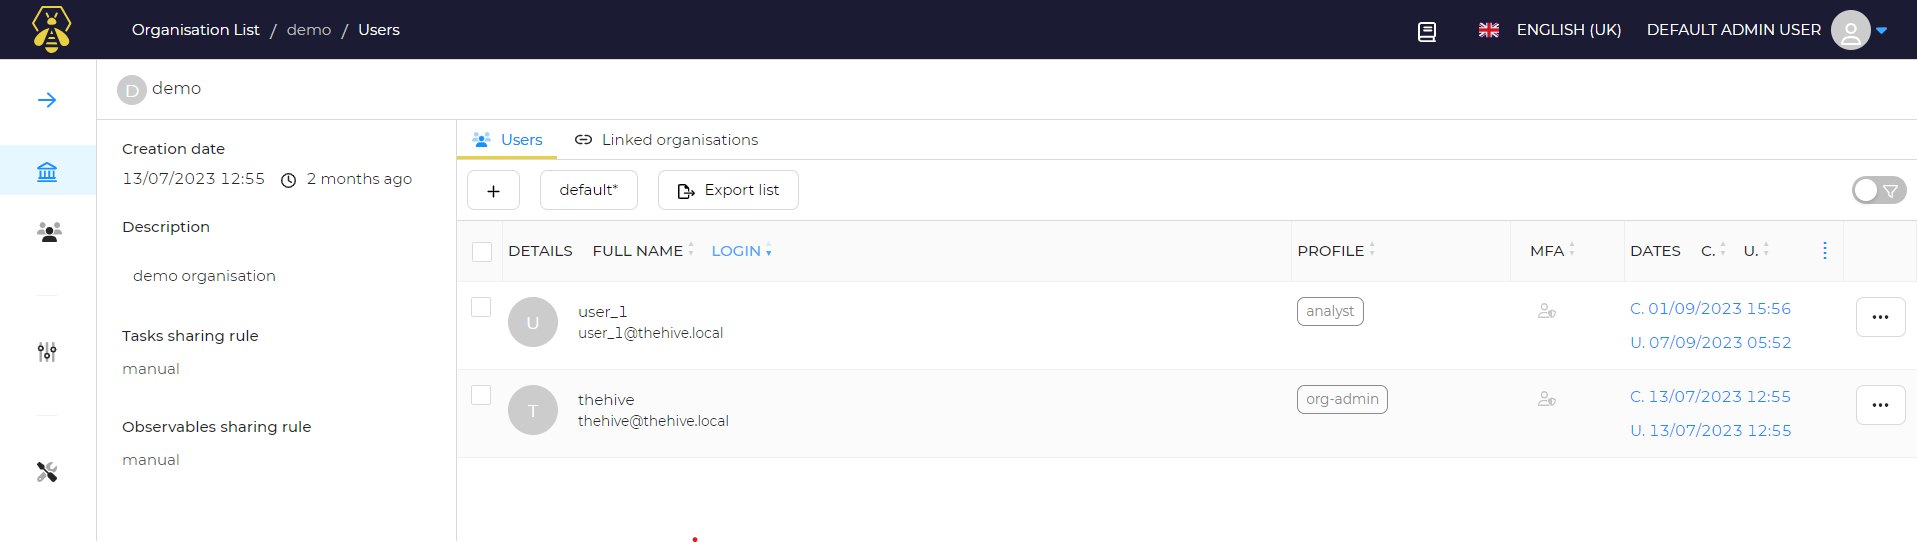
\includegraphics[scale = 0.28]{Organization_1.png}
    \caption{Organization dashboard}
    \label{fig:Organization dashboard}
\end{figure}

    
\begin{justify}

Here, in the above image an admin logged in whose name is "DEFAULT ADMIN USER"
and he creates an orgnization named "demo" .In "demo" organization he creates two users.He can add more user by clicking "+" sign . After clicking "+" sign the following dialogbox will be shown to provide user information.After filling up the dialog box with user information and clicking on "Confirm" ,a new user will be added to organization
%image
           
\end{justify}


\end{frame}


\begin{frame}{Organization continued}

\begin{figure}[htp]
    \centering
    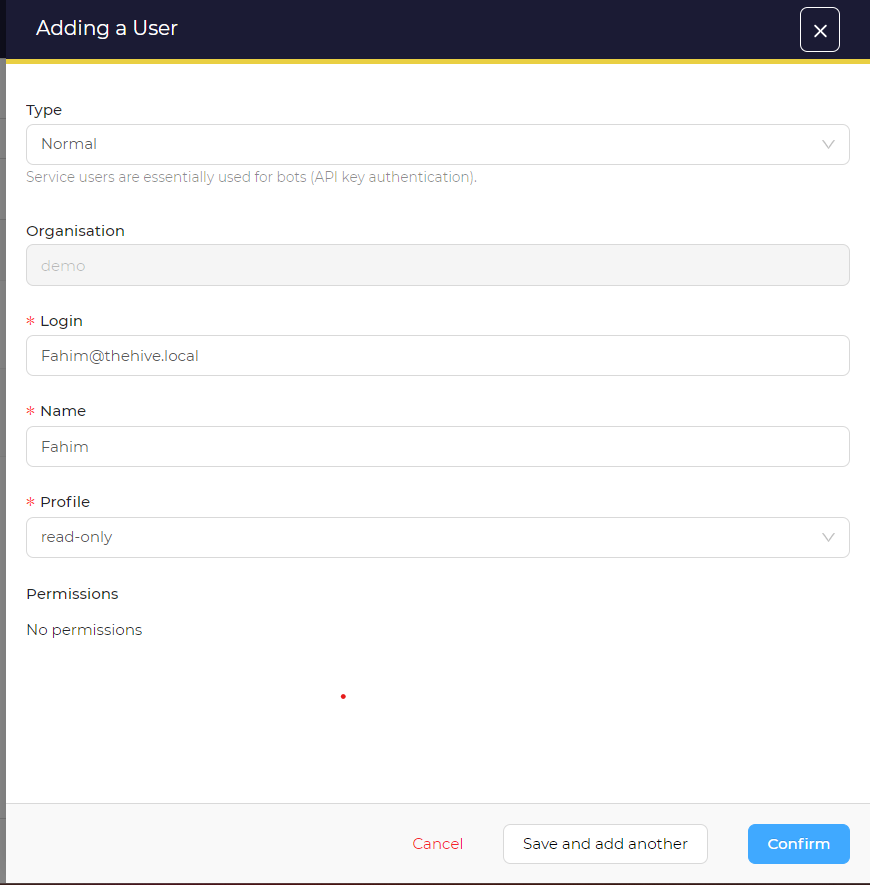
\includegraphics[scale = 0.28]{Organization_2_adding_a_user.png}
    \caption{Adding a user}
    \label{fig:Adding a user}
\end{figure}
        
\end{frame}


\begin{frame}{Cases}
\begin{justify}

Users of an organization with analyst or org-admin role can create cases at the response of any security incident and Other users can see the case and deal with the cases collaboratively.

After logging into an user account ,a user can see the list of cases of his organization .
\begin{figure}[htp]
    \centering
    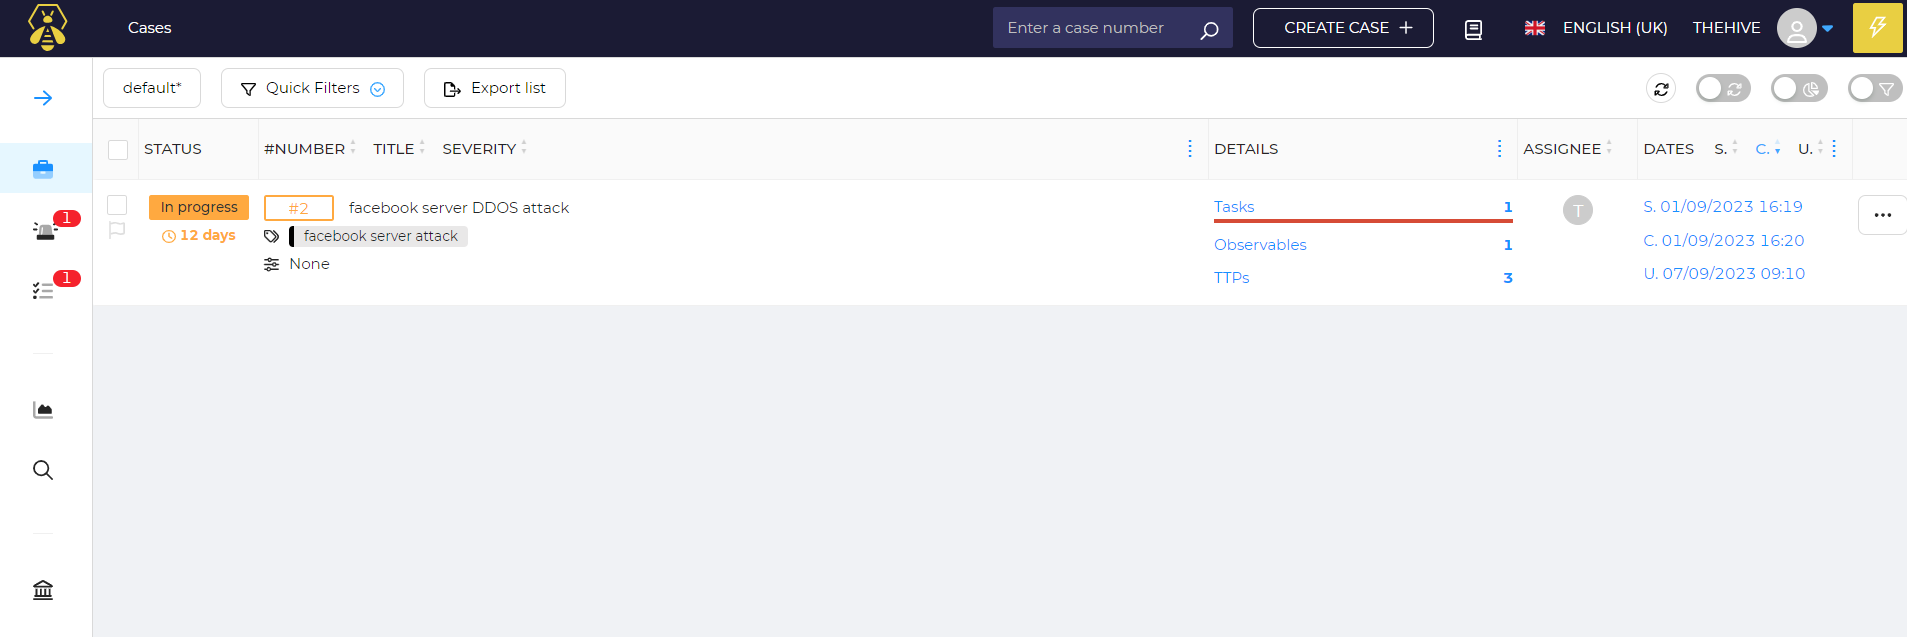
\includegraphics[scale = 0.28]{User_home_page.png}
    \caption{User dashboard}
    \label{User dashboard}
\end{figure}


\end{justify}

\end{frame}

\begin{frame}{Cases continued}

To create a new case a user can click on "CREATE CASE +" button on the top and then the following dialogbox will be shown
\begin{figure}[htp]
    \centering
    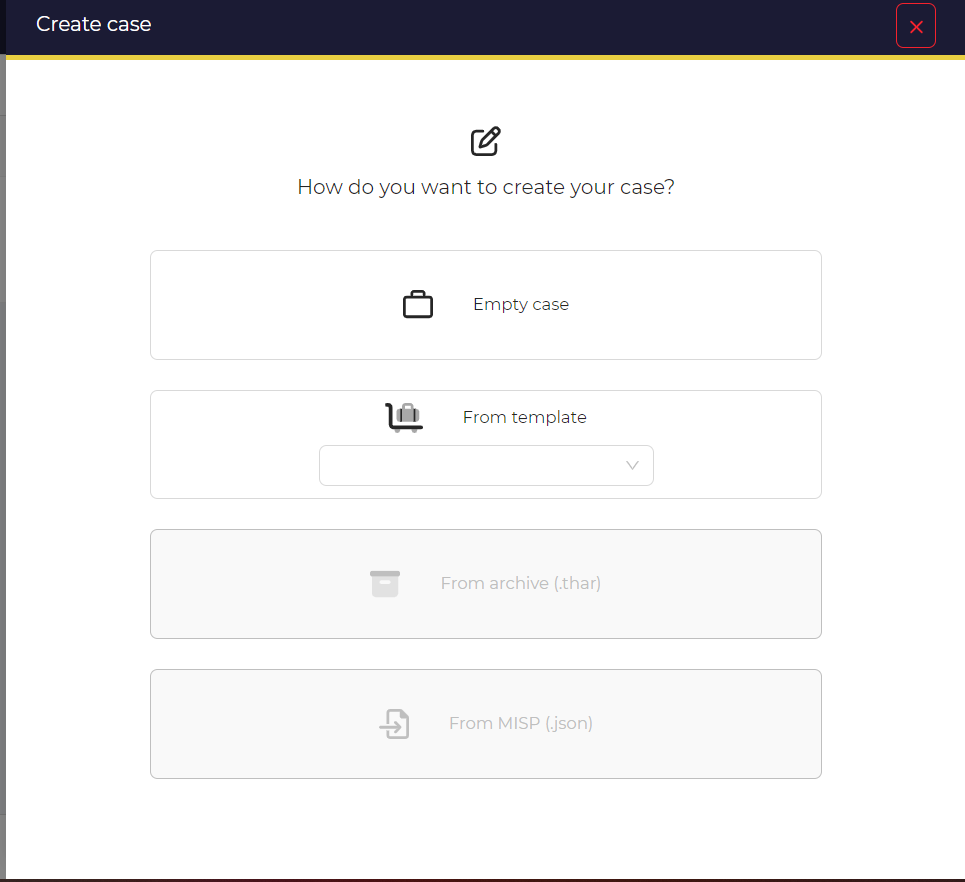
\includegraphics[scale = 0.28]{creating case(empty or template).png}
    \caption{Choose case type(Empty or template)}
    \label{Choose case type(Empty or template)}
\end{figure}
    
\end{frame}


\begin{frame}{Cases continued}
\begin{justify}

From above user can select "EMPTY" to create a case from scratch or he can import a security event as a case from "MISP" after selecting "template" 
option

After selecting "EMPTY" the follwing dialog box will be shown
\begin{figure}[htp]
    \centering
    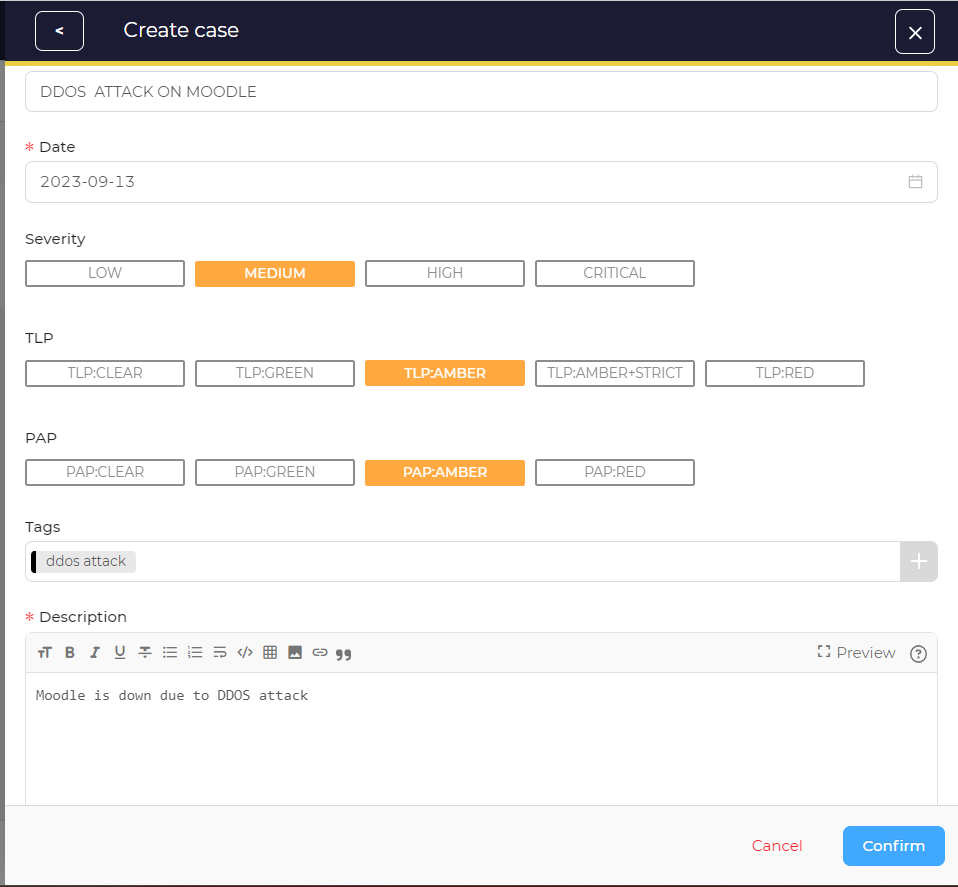
\includegraphics[scale = 0.28]{Craete empty case.png}
    \caption{Creating a case}
    \label{Creating a case}
\end{figure}


\end{justify}

\end{frame}

\begin{frame}{Cases continued}
  Then after filling the dialog box with the information of security incident,when he clicks on "Confirm" a new case will be added to its organization and the case will be seen by other users of this organization.
\begin{figure}[htp]
    \centering
    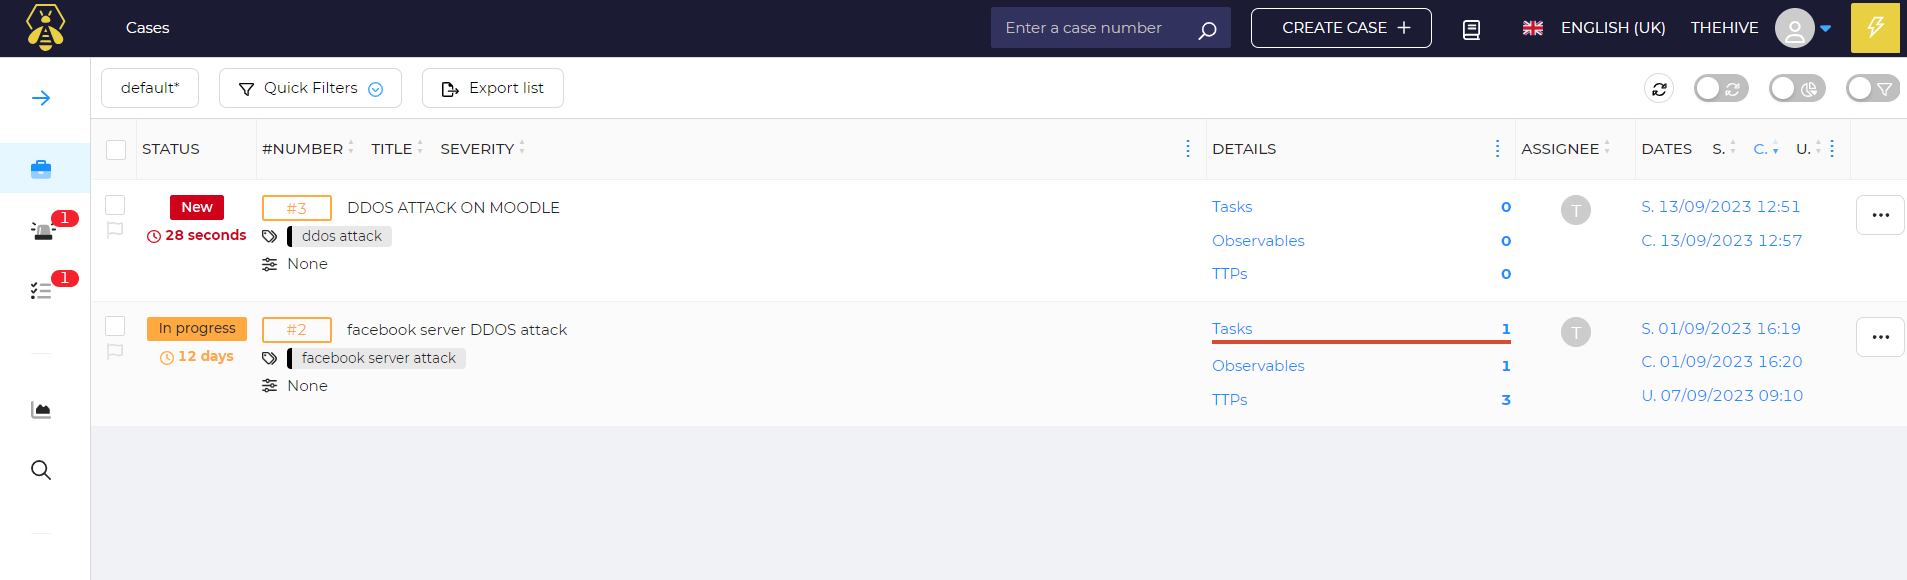
\includegraphics[scale = 0.28]{New case added.png}
    \caption{User dashboard(after creating a case)}
    \label{User dashboard(after creating a case)}
\end{figure}
    
\end{frame}


\begin{frame}{Task}
\begin{justify}
After creating a new case ,a user can create tasks which should be performed to resolve the case and assign those tasks to different users.
So,For a particular case  while adding a task we need to fill up the following dialogbox with necessary information about that task
\begin{figure}[htp]
    \centering
    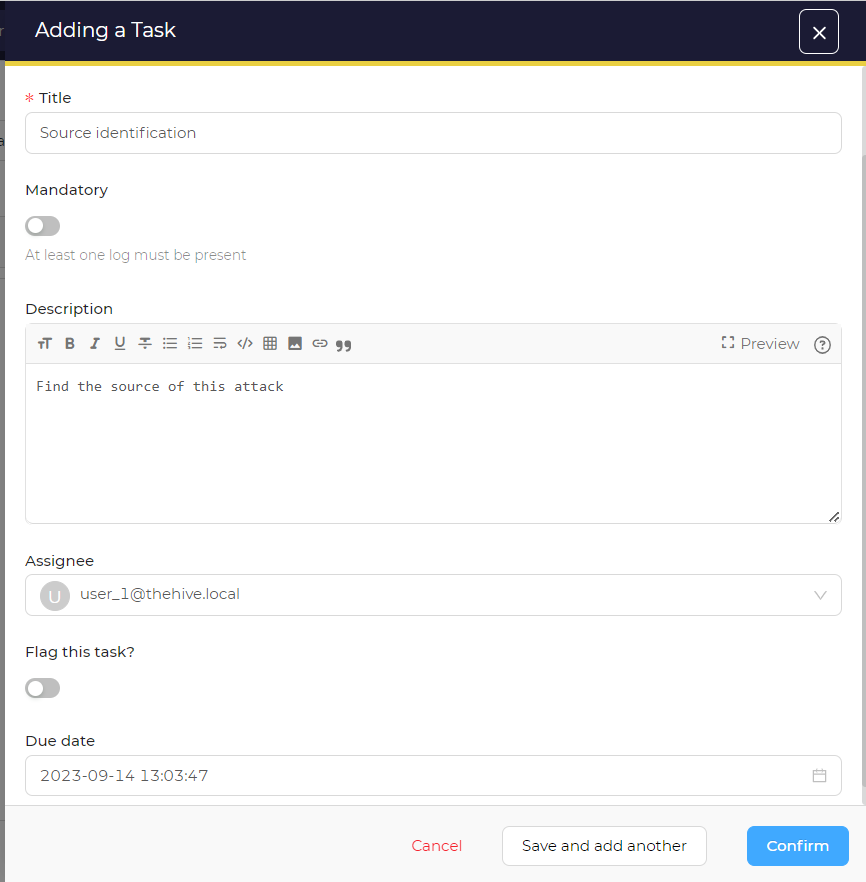
\includegraphics[scale = 0.28]{Adding a task.png}
    \caption{Adding a task}
    \label{Adding a task}
\end{figure}


\end{justify}

\end{frame}

\begin{frame}{Task continued}

Then after creating a task successfully the dashboard of a case under "Tasks" tab will look like below
\begin{figure}[htp]
    \centering
    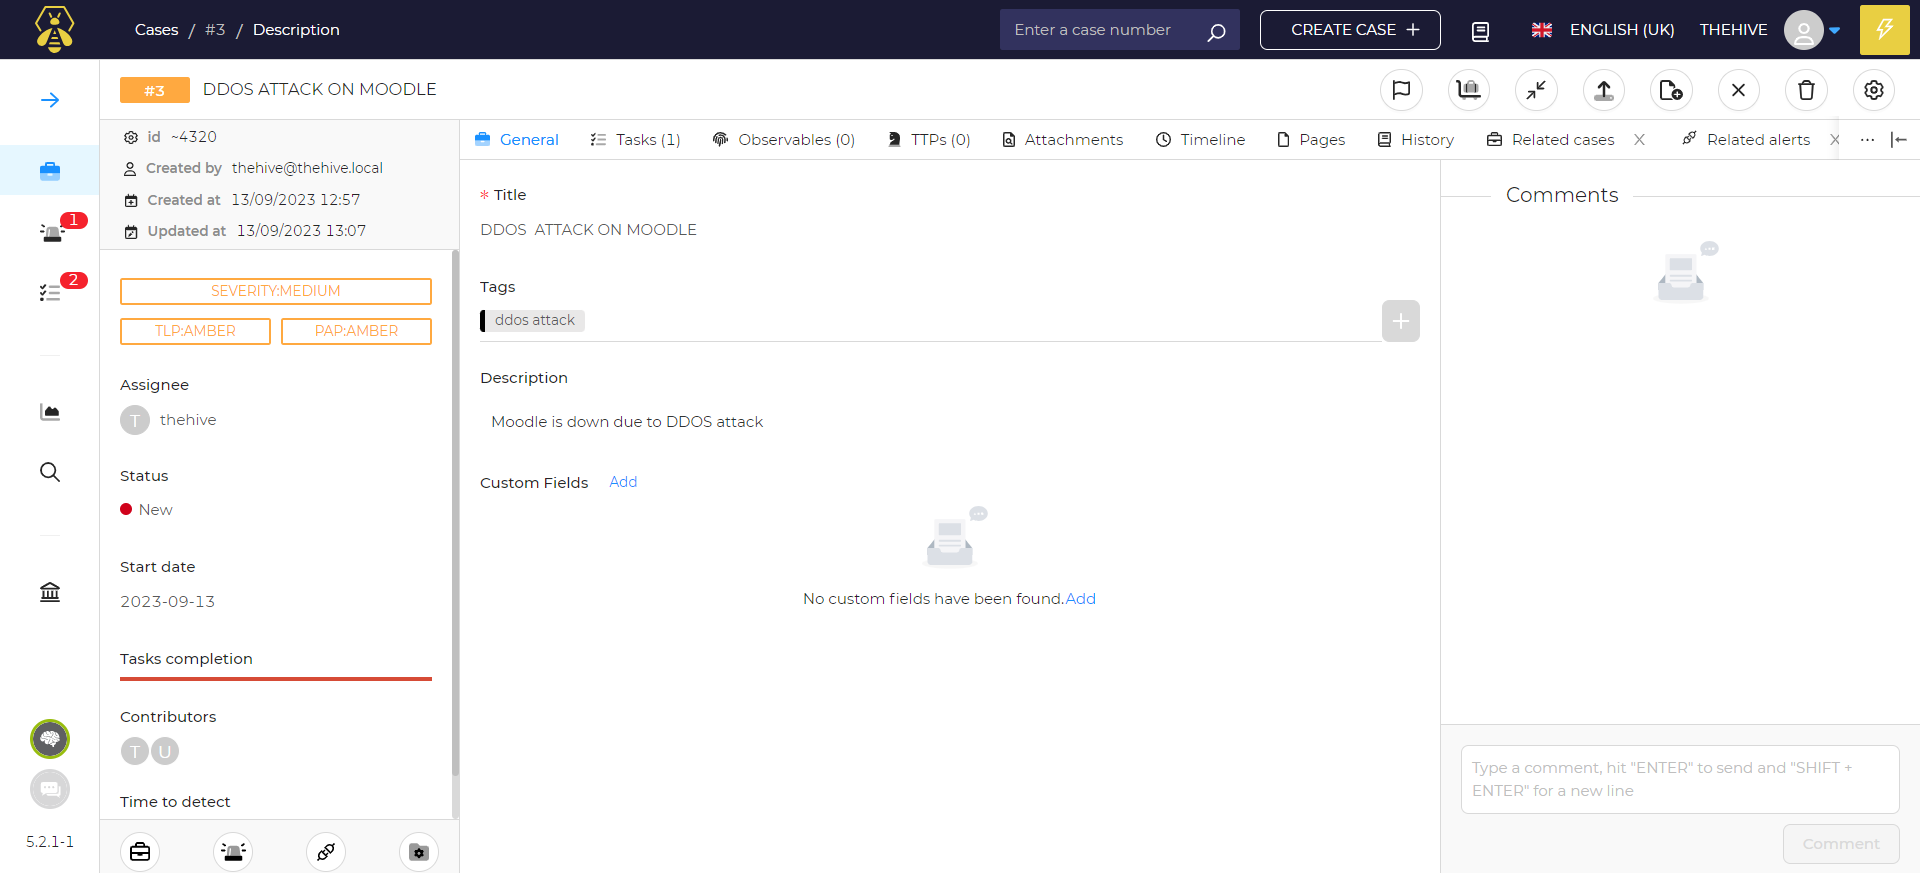
\includegraphics[scale = 0.28]{case dashboard.png}
    \caption{Case dashboard(after adding a new task)}
    \label{Case dashboard(after adding a new task)}
\end{figure}

    
\end{frame}



\begin{frame}{Observable}
\begin{justify}
Observables are the elements of a case on which the user(security analyst) will report their analysis(e.g. ip address, hash of malicious file)

\end{justify}

\end{frame}


\begin{frame}{Observable continued}
\begin{justify}

For a case a user can add one or more observables.To add a new observable a user need to fill up the following dialog box.
\begin{figure}[htp]
    \centering
    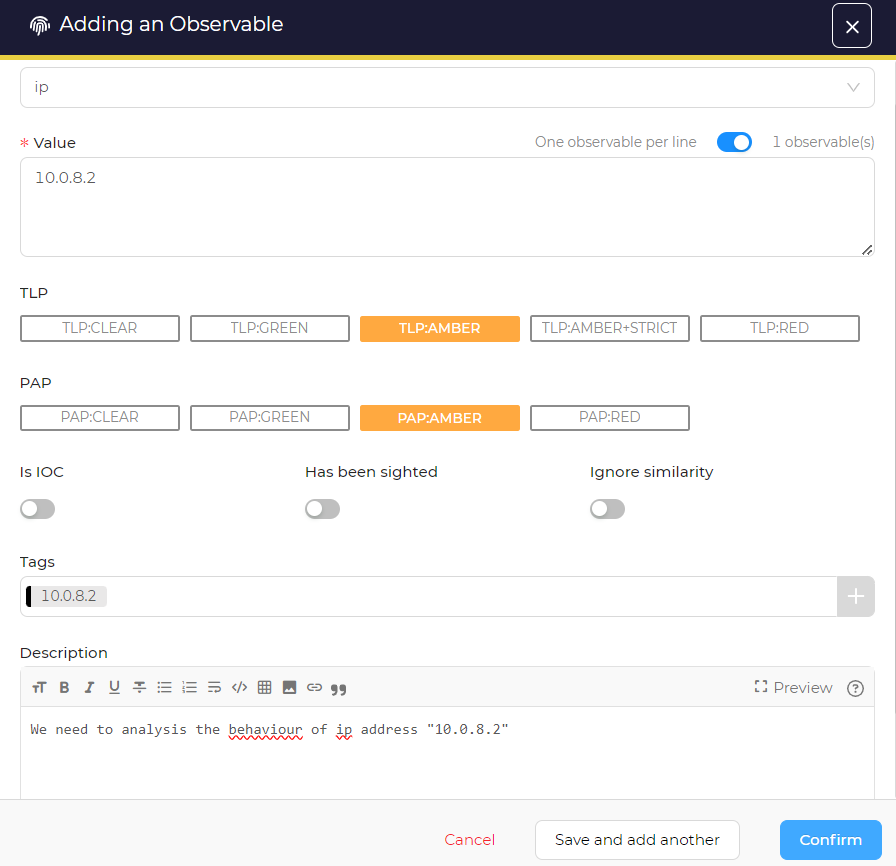
\includegraphics[scale = 0.28]{Adding a observable.png}
    \caption{Adding an observable}
    \label{Adding an observable}
\end{figure}


\end{justify}
    
\end{frame}


\begin{frame}{Observable continued}
After adding an observable successfully, the dashboard of a case under "Observables" tab will look like below

\begin{figure}[htp]
    \centering
    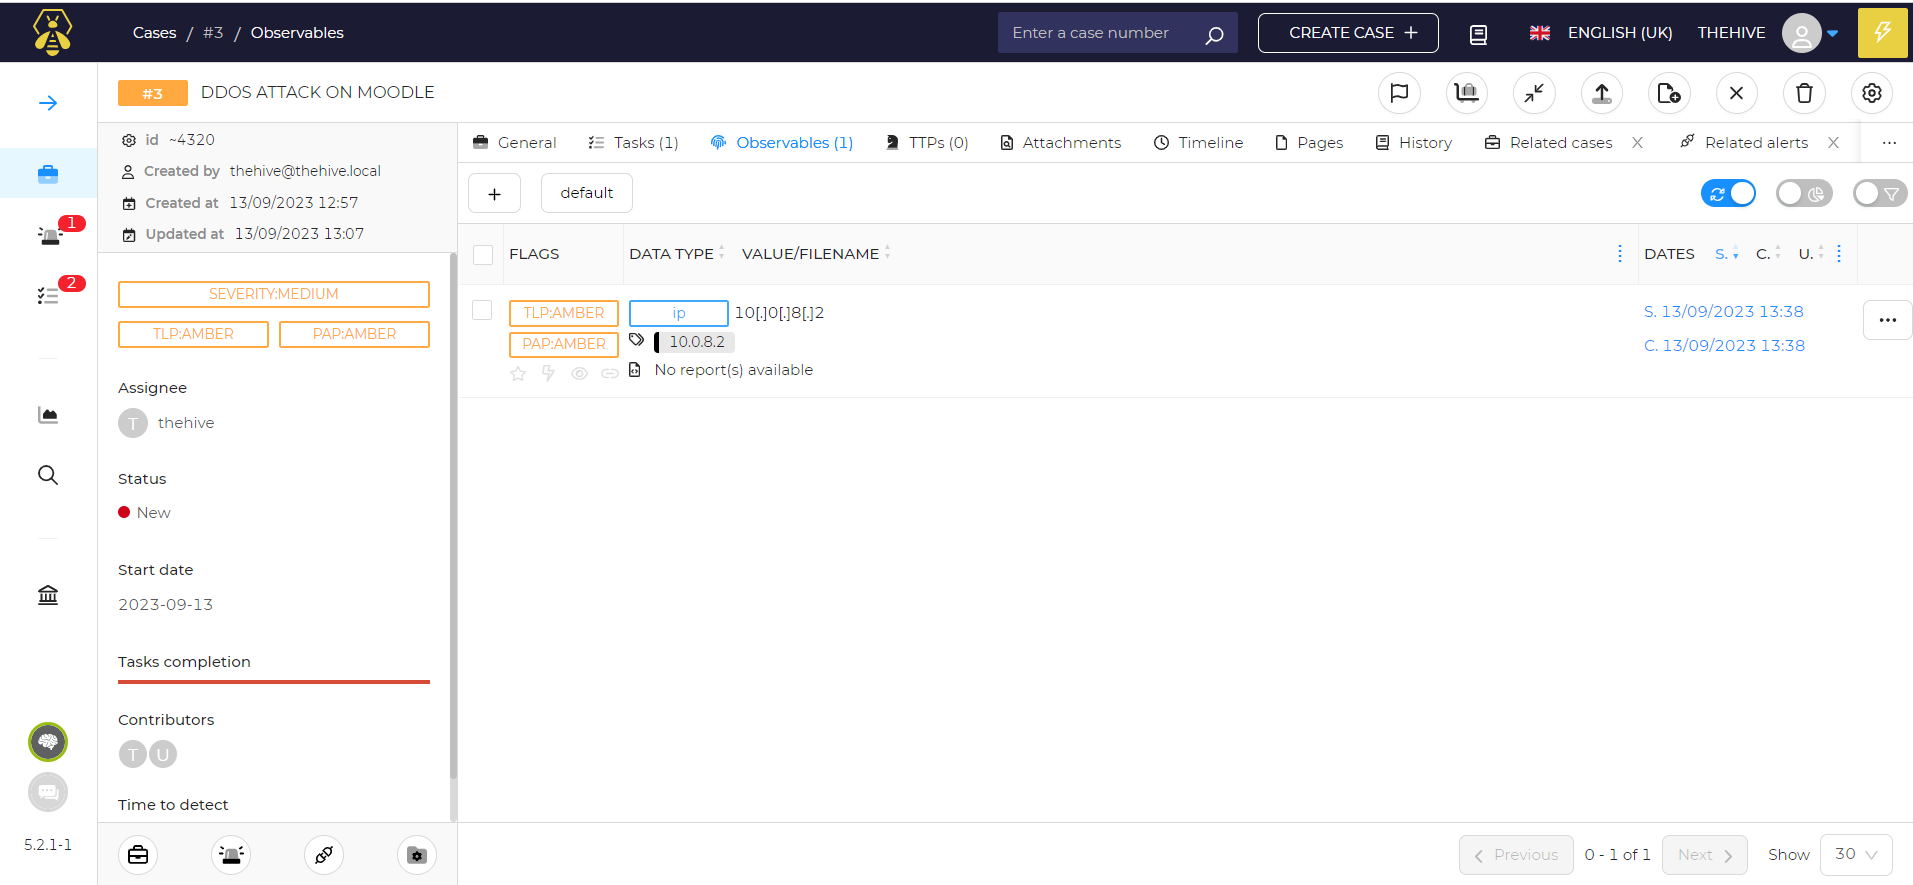
\includegraphics[scale = 0.28]{case dashboard after adding an observable.png}
    \caption{Case dashboard(after adding a new task)}
    \label{Case dashboard(after adding a new task)}
\end{figure}
    
\end{frame}


\begin{frame}{Observable continued}
\begin{justify}
Then after adding observables for a case ,the analysts can report their analysis on these observables by doing analysis manually or he can automate the process of analysis with the help of "CORTEX". 
\end{justify}

\end{frame}









